\chapter[Integrating Free and Open Source Solutions into Geospatial Science Education]
{Integrating FOSS into Geospatial Science Education}
\label{app-b}

\textbf{Reprint}

Vaclav Petras, Anna Petrasova, \textbf{Brendan Harmon}, Ross Meentemeyer, and Helena Mitasova. 2015. Integrating Free and Open Source Solutions into Geospatial Science Education. \emph{ISPRS Int. J. Geo-Information} 4, 2 (2015), 942–956. DOI:url{http://dx.doi.org/10.3390/ijgi4020942}

\textbf{Attribution}

Vaclav Petras and Anna Petrasova
developed this approach,
implemented methods 
for building course web pages,
and wrote this paper.

I developed and taught the course 
\emph{LAR582: GIS for Designers},
wrote the section about this course,
and edited the paper.

Ross Meentemeyer
directs the MGIST program at the Center for Geospatial Analytics at
North Carolina State University. 
He contributed to this paper with advice, guidance, support, and editing.

Helena Mitasova
pioneered this approach,
developed and taught the courses 
\emph{GIS/MEA582: Geospatial Modeling and Analysis} and
\emph{GIS595/MEA592: Multidimensional Geospatial Modeling},
wrote the sections about these courses,
and edited the paper.

\vfil
\pagebreak

%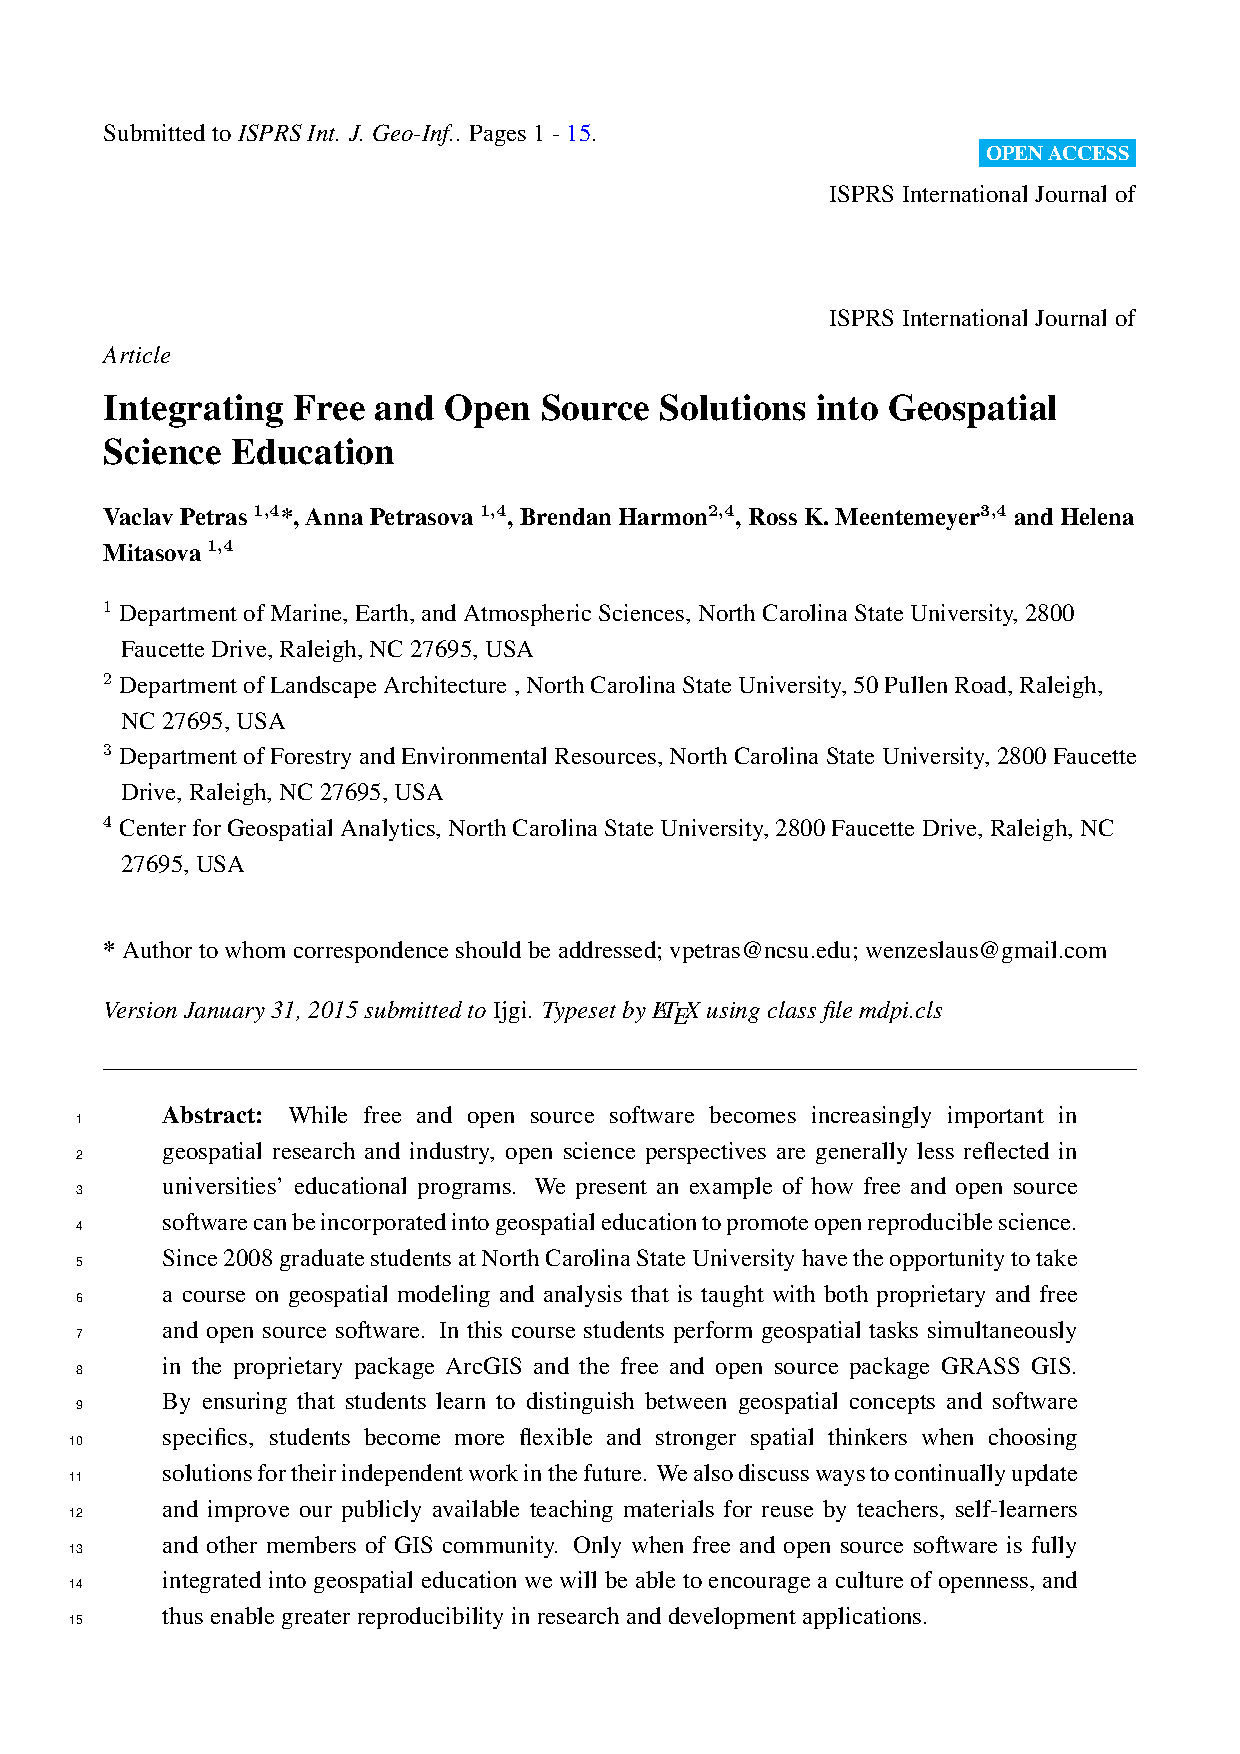
\includepdf[pages={-}]{integrating-free-open.pdf}


